% \documentclass[12pt,a4paper]{article}
\documentclass[12pt]{article}
\usepackage[left=1in, right=1in, top=1in, bottom=1in, includehead=false, includefoot=false]{geometry}
\usepackage{url}

\usepackage[utf8]{inputenc}
\usepackage{caption}
\usepackage{subcaption}
\usepackage{natbib}
\usepackage{epsfig,graphicx}
\usepackage{float}
\usepackage{chngpage}
\usepackage{multirow}
\usepackage[hidelinks]{hyperref}
\usepackage[none]{hyphenat}
\usepackage[all]{nowidow}
\usepackage[dvipsnames]{xcolor}
\usepackage{bm}
\usepackage{soul}
\usepackage{textcomp}

\usepackage{times}
\usepackage{xcolor}

\urlstyle{rm}

% \usepackage{float}
% \restylefloat{table}

\bibliographystyle{chicago} % agsm
% \bibliographystyle{../style/chicago}

\graphicspath{{../figures/}}

\captionsetup{%
   justification=raggedright
}

% \usepackage[doublespacing]{setspace}
% \usepackage[document]{ragged2e}
% \setlength{\RaggedRightParindent}{\parindent}

\setlength{\bibsep}{0pt plus 0.5ex}
\newlength{\li} \setlength{\li}{12pt}
\newlength{\si} \setlength{\si}{.4in}
\setlength{\parindent}{\si}
\setlength{\parsep}{0pt}

\makeatletter
\newcommand\iraggedright{%
  \let\\\@centercr\@rightskip\@flushglue \rightskip\@rightskip
  \leftskip\z@skip}
\makeatother

\newcommand{\redtxt}{\textcolor{red}}

\date{}


\title{Identifying spatial patterns on choropleth maps: A comparison between humans and deep learning models}

% \title{How Well Computers Can Read Spatial Patterns using Visual Symbols in Choropleth Maps Compared with Humans}

\begin{document}
\iraggedright
\maketitle

\section{Study Objectives}




% \section{Background and Rationale}

% A map is the graphic representation of the environment \citep{robinson1995elements}. With the development of free map making tools, making digital maps are more accessible than ever \citep{Robinson2019}. The Internet represents a new medium for cartography with the seemingly limitless range of online map products available \citep{peterson2005maps}. The increasing quality and availability of the digital maps is now providing a realistic alternative to the traditional paper map format \citep{Hurst2013}. An increasing proportion of mapping contents are being presented and consumed by use of a digital interface of some description \citep{dodge2011mapping}. For example, the famous traditional media such as New York Times and Forbes use digital maps on the websites to help convey their opinions. Digital maps including online map images have evolved in recent years to become a part of our everyday life \citep{Aly2017}. 

% There are different types of online maps including thematic maps to display a spatial phenomenon (i.e., theme) using different visual symbols. Thematic maps can be further divided into categories such as choropleth maps. In the research, we focus on choropleth maps, which are a type of the most commonly-used thematic maps. In a choropleth map, enumeration units (such as states in a state-level choropleth map of the United States) are filled with different colors, which are the visual symbols used in choropleth maps. Each color represents a value range of the measurement of a map theme such as population density \citep{slocum2009thematic}. The colors in choropleth maps show different spatial patterns of the presented phenomenon. 

% Spatial pattern is the description for the arrangement or placement of geographic features \citep{kimerling2016map} such as how the trees in the Oval on the Ohio State campus are distributed. We select two common spatial patterns in this study for computers and humans to read:(1) whether the represented phenomenon concentrated or clustered in some area and (2) whether the values tend to occur near their similar vlaues or different values. 

% But maps are not designed for computers to read, so it can be difficult for computers to read and comprehend maps. In this protocol, reading maps by computers means computers can tell us what is on the map, for example, whether the represented phenomenon concentrated or clustered in some area. Computers operate on a different system and may need a leap of faith to read maps. Nevertheless, intelligent machines that can understand artifacts (including maps) seem to be trending toward being part of our future \citep{cascio2016technology} and exploring such a future in map making is interesting and exciting. 

Maps are artifacts made by humans and, more importantly in this context, {\it for} humans to read. As a consequence, maps are an effective means of presenting spatial patterns \citep{kimerling2016map}. Humans develop map reading skills \citep{presson1982development,gilhooly1988skill} to comprehend spatial patterns from the map naturally. Reading maps has been challenging, if not impossible, for traditional computer algorithms. In recent years, however, dramatic progress has been made in computer vision. Thanks to the advances in deep neural networks \citep{Szeliski2021}, methods in computer vision have been successfully applied to problems in various domains where images need to be recognized or classified. For example, in facial recognition, deep learning models are applied on a face photograph database designed for studying the problem of unconstrained face recognition and have achieved an accuracy that approaches or is even beyond humans \citep{Wang2021}. Our own preliminary research has also shown that deep learning models can be used to successfully identify maps and map elements such as areal symbols, titles, and legends. While we can agree that artificial intelligence may not have reached a point that machines can read maps as humans do, would it be possible that computers can recognize some contents of maps utilizing the cutting-edge algorithms in computer vision and then do some analysis and therefore can recognize spatial patterns presented on the map?

The goal of the overall study is to explore how well artificial intelligence algorithms can compare with humans in identifying spatial patterns in a specific type of maps: choropleth maps. Popular in a wide range of applications, a choropleth map is used to display the spatial distribution of quantitative data across the enumeration units such as counties and states in a region. A common approach to making this type of map is to group the data into a number of classes and a color is used to represent a class. In other words, each unit is rendered using areal symbol (i.e., the shape of the unit filled with a color). These symbols hold the key to understand the spatial pattern of the data. For example, the following is an example map that will be used in this study and one should recognize a unit with a certain value on the map tends to associate with units with similar values because similar colors tend to be close to each other. One of the major goal of representing the data using such a map is to allow readers to recognize such patterns. In the past three years, we have been developing deep learning to identify symbols from choropleth maps and the results can be used to analyze spatial patterns on the map using existing algorithms. It is possible to assemble computer programs that can be used to automatically identify the spatial patterns on the map, and we are interested how such computer programs can compete or compare with humans.

\begin{figure}[!ht]
    \centering
    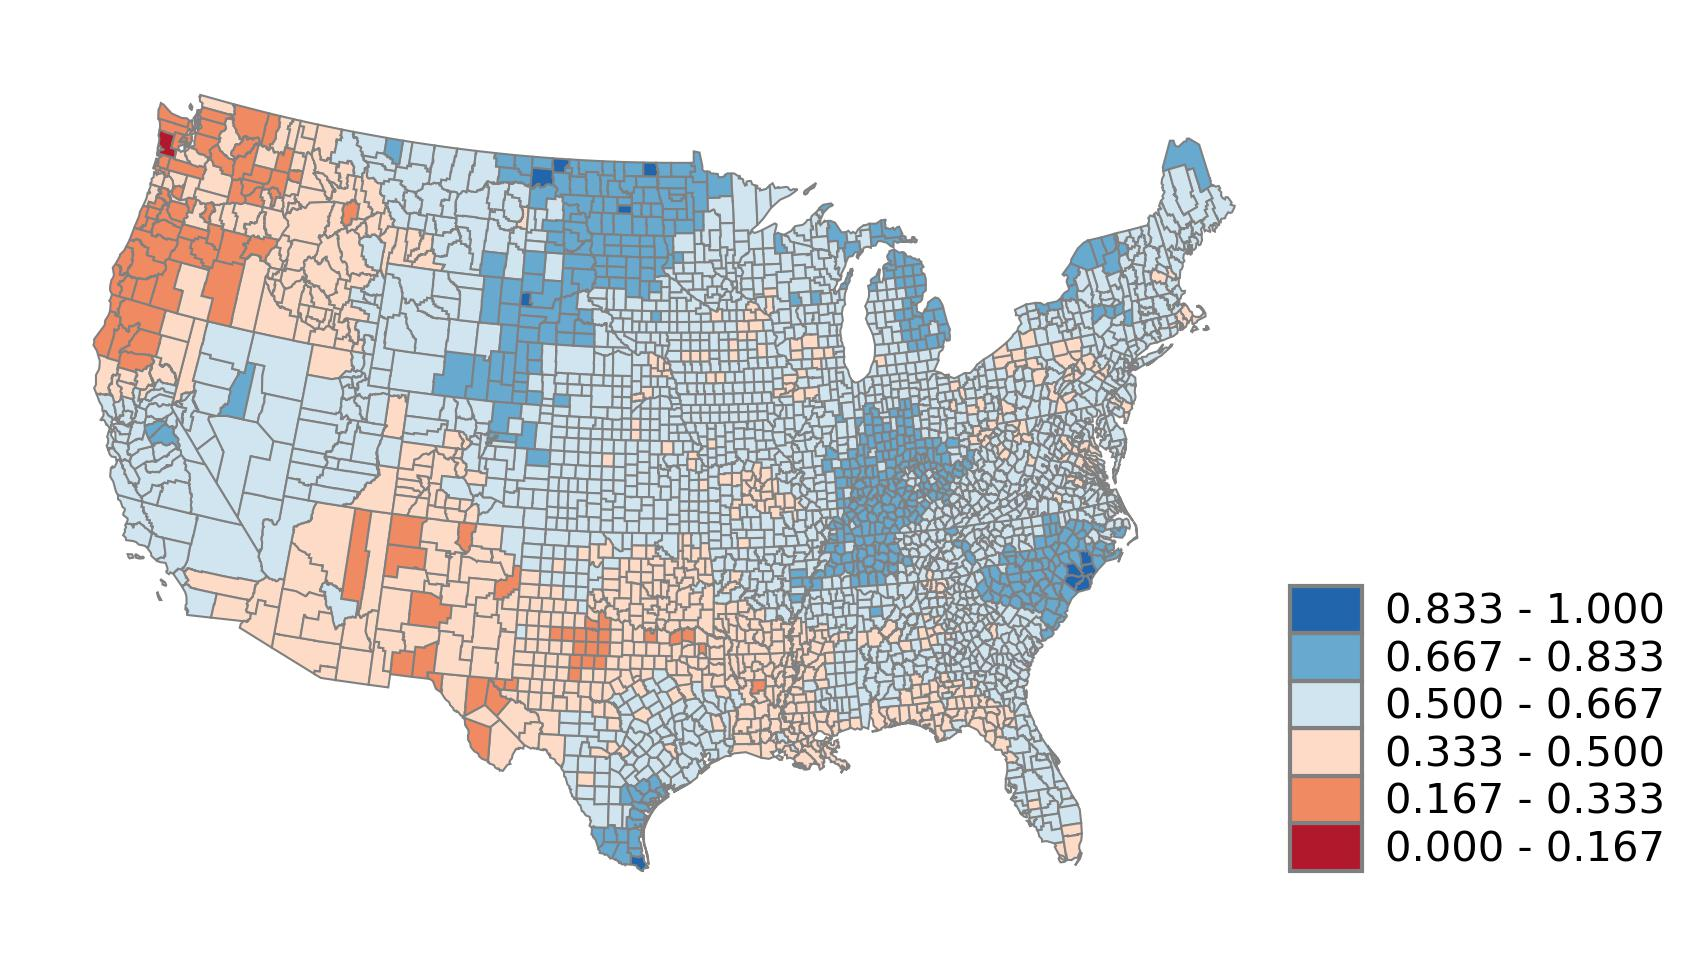
\includegraphics[width=0.9\textwidth]{us_RdBu_6_pos_large.jpg}
    \caption{An example map that will be used in this study.}
    \label{fig:MLP}
  \end{figure}

In order to conduct the comparative study, it is critical to understand how humans perform on reading spatial patterns on the map when the exact same map will also be processed by computer programs. On the computer side, deep learning-based object detection models in computer vision will be used to detect the mapping area of a choropleth map, and then algorithms in traditional computer vision, data mining, and spatial analysis will be applied to extracting more information from the mapping area and analyzing its spatial patterns. On the human side, we intend to conduct surveys that use the same set of maps that will be used by the computers to ask our subjects if they can recognize the patters presented on the maps. In this protocol, we detail the design and procedures of the surveys. We do not need and will not record personal identifiable information in this study.

% \section{Procedures}

\section{Research design}

% This is a study to measure how well humans can read spatial patterns using visual symbols in choropleth maps. 

We will conduct surveys that ask participants questions about spatial patterns on a series of choropleth maps. For a given map, we focus on two kinds of spatial patterns that can be observed from choropleth maps by asking each participants two questions:

\begin{enumerate}
    \item Is the phenomenon represented by the visual symbols (colors) concentrated in some area or scattered over the map? 
    \item Do the values tend to occur near their similar values or different values? 
\end{enumerate}

For each question, we will present two options of either yes or no. While there are different kinds of spatial patterns, these two types (concentration and association) illustrate meaningful and typical information that can be observed on a choropleth map. In addition, we can develop computer programs to answer exactly the same questions. This will provide a common basis for our comparative study on spatial pattern recognition using choropleth maps between humans and computer algorithms.

We will design our maps to facility the questions. Each map will only have two visible elements: the mapped area where the spatial units are rendered, and a legend. In other words, the maps used for our surveys will be different from the "normal" maps that would have a title and other elements. Because our study will focus on how humans and computer programs can use symbols (colors, in this specific case) to understand spatial patterns on choropleth maps, the way the maps are designed will make sure the symbols are the focus during the survey. Our computer program will be build specifically to recognize and analyze the mapped area and legend. Our maps will vary in the following aspects:

% The difficulty to read choropleth maps can be affected by different variables. We use maps with different design variables in the survey to test the human performance for different levels of reading difficulties. In order for better control of the design variables, we synthesize choropleth maps for testing. The synthetic maps are not normal map as we see in daily lives. The purpose of this experiment is to understand how visual symbols (colors) can be used to identify spatial patterns. So, we removed titles, legend headings, only the visual symbols are presented.

\begin{itemize}
    \item {\bf Base map.} We use two sets of spatial units to provide different levels of cognition challenges. The first is based on the 88 counties in Ohio, and the second are the 3,109 counties for the conterminous United States.

    \item {\bf Data.} The spatial data used in synthetic maps present different spatial patterns for our subjects to recognize. We synthesize spatial data for the two base maps with four types of spatial autocorrelation: negative spatial autocorrelation, no spatial autocorrelation, small positive spatial autocorrelation, and large positive spatial autocorrelation.

    \item {\bf Number of classes.} In general, a choropleth with a high number of classes may provide more detailed information while making it difficult for us to read. On the other hand, it is reasonable to assume that computers would not have a problem with the number of classes, but identifying the colors on the map may be more of a challenge for the computer. The cartography literature generally suggest a relatively small number of classes, such as 5. We will use three different numbers of classes: 4, 6, and 8 to render each map.

    \item {\bf Color scheme.} The set of colors used for the classes on a map is called a color scheme. Color schemes vary based on what kind of colors are used and how the differ. We will use two color schemes: a sequential color scheme where color range from light blue to dark blue, and a red-yellow-blue diverging color scheme where dark blue and dark red on both ends progress to light blue and yellow, respectively, toward the middle of the scheme. These are all colorblind safe schemes as suggested by ColorBrewer\footnote{https://colorbrewer2.org/}, the defacto color standards for cartographers and beyond \citep{harrower2003colorbrewer}.
\end{itemize}

% Different base maps with different number and sizes of enumeration units are the first variable for the reading difficulty. Because the number and size of enumeration units can influence the reading difficulties of humans. If the relative size of enumeration units is small and there are many units in mapping area, it is more difficult for humans to process the information. If there are only a few enumeration units with large sizes, humans should be easy to recognize the presented information. Therefore, in our study, we adopt two base maps: maps for Ohio at county level (easy) and maps for contiguous United States at county level (difficult). 

% The second design variable is the color scheme. We apply color schemes suggested by ColorBrewer\footnote{https://colorbrewer2.org/} to color the enemeration units in the two base maps. ColorBrewer is a simple online tool that helps map designers choose appropriate color schemes to use in their maps. We synthesize maps with sequential and diverging color schemes. For each color scheme, we  select 3 different numbers (i.e., 4, 6, and 8) of colors used in one map. The types of color schemes and number of colors can also influence the difficulties of map reading. For example, it is easier to recognize relationships between high and low values if a diverging color scheme is used. And when there are many colors (>=8) used in one map, map users will find it difficult to read even though a sequential or diverging color scheme is used.

In sum, each map will be defined by its base map (Ohio or the U.S.), color scheme (sequential or diverging), number of classes (4, 6, or 8), and spatial pattern (negative, random, small positive, or large positive associations). We will make two copies of each combination (the data are randomly generated). Therefore, we have a total of 96 maps, or 2 (base maps) x 2 (color scheme types) x 3 (numbers of colors) x 4 (spatial patterns) x 2. In the survey, we will allocate 16 map images with two questions for each to one participant. It will take one participant about one minute for one question. They will spend about 20 minutes on the survey. The answers from our subjects will be collected using Qualtrics survey reports, which will then be analyzed (see below).


\section{Sample}

We plan to recruit approximately 75 adult participants (age 18-65) from Ohio state students, faculty, and staff members to answer the questions in our survey. The survey will be distributed in two undergraduate classes in the Department of Geography: Design and Implementation of GIS (GEOG 5223) and GeoVisualization (GEOG 5201). Students are not required to take this survey. Those who do take the survey will receive bonus participation points. In addition, We will use online bulletin boards, email mailing lists, in-class announcements, and personal contacts to reach out to potential participants. 

\section{Measurement and Instrumentation}

We will use Qualtrics to conduct our surveys. To conduct the experiments, each participant needs a computer system (including a monitor and a mouse). All experiments will be done online through using a web browser. The application can start the experiments at any time or at any place without log-in requirements. Data will be saved on the server of Qualtrics, which can be retrieved for further analysis. All the data collected here is anonymous, and no identifiable information will be recorded. The surveys are conducted on the platform of Qualtrics, and the choropleth map images are synthesized by Python. 

The experiments will evaluate the reading performance of participants on spatial patterns in choropleth maps using choropleth maps. For each question, the participants will be asked to select one from the choices. The answers will be saved in a survey report of the Qualtrics platform. Then, the accuracy rates for the questions of maps will be calculated. The accuracy rates will be compared with rates by computers.

\section{Procedures}

Each participant will be asked to take the survey in a safe environment with relatively low ambient noise. Each survey contains four sections: informed consent form, instruction, background information, the two question, and a random completion code generated at the end for the undergraduate students from the two geography classes.

\begin{itemize}
    \item The informed consent form explains the the goal of the study, procedures and tasks, risks and benefits, confidentiality, and participant rights. Our participants will have a basic understanding of this project, then they can decide to continue the survey or not. 
    
    \item The instruction section introduces what the participants will see and what they should do during the survey. An example of a map with the two questions is included in the instruction. After this section, the participant should know what to do during the experiment. 

    \item In the section of background information, the participant will be asked to answer their background in geography and cartography, which will be used for experiment control purposes. 

    \item In the question section, the participant will be presented a series of choropleth maps with different spatial patterns and be asked the two questions about spatial pattern for each map. They should read the maps carefully and answer the questions based on what they read and learn from the mapping areas. Each participant will be asked to view 16 maps.

    \item At last, a random completion code will be presented to students in the two geography classes (GEOG 5223 and GEOG 5201) mentioned above. The completion code will be used as the proof of completion for bonus credit. The code is randomly pulled from a pool of codes that are prepared beforehand. The codes do not contain any personal information and are not associated with the participants in any manner. In other words, given a code we cannot trace back to the survey and questions answered by the participant, or vice versa. In this way, personal information of the participants will not be identified.
\end{itemize}

\subsection{Internal validity}

The surveys are designed to measure the ability of participants in identifying spatial patterns. The two questions about spatial patterns of the phenomenon presented on a map are non-trivial. They represent the reason why maps are useful: to learn how things distribute on space. These questions require participants to read the symbols on the map carefully to recognize the patter. The participants will be asked to take the survey in a relatively quiet environment without disturbs. And the devices especially monitors should be of good quality to display choropleth maps with no significant color differences. 

The experiment will not discriminate against any population and will be open to all on a voluntary basis. We use colorblind safe color schemes as suggested by extensive research behind colorbrewer \citep{harrower2003colorbrewer}. This experiment utilizes a forced choice response in which the correct choices in the experiments are predefined by the researchers. We will also make some slides with instructions to introduce the experiments and how the Qualtrics survey will work. By using the instructions, we expect the participants will be familiar with the general process of the experiments and then concentrate on the experiments when they start. 

\subsection{Data handling analysis}

Data would be collected by asking participants to read maps and answer questions. Key personal information such as name and personal email would not be collected. The random completion code is generated by the Qualtrics platform and this code does not contain any personal information. Thus, we as researchers would not be able to know the workers' key personal information such as name and cannot identify who they are behind the screen. Thus, subjects are actually totally anonymous during the whole research process and subject confidentiality would therefore be ensured throughout the whole experiment.

The average correctness rate of the responses with respect to different base maps and color schemes will be used to reveal the impacts of the variables on the reading performance of our subjects. We will also develop statistical models to understand the relationship between the human reading performance on choropleth maps and the map design variables and spatial patterns. We will run our computer programs to answer the exact same questions (the program will output yes or no for each map and each question). As a final step of this study, we will compare the human responses with those from the computer. The results of this comparison will shed light on how close today's computer based algorithms can compete with humans in reading spatial patterns on choropleth maps. 

% \section{bibliography}

% \printbibliography %Prints bibliography
\bibliography{references}


\end{document}
